\section{Linjärkombinationer}
    \paragraph{Definition} Låt $V$ vara en mängd vektorer och $v_{1}, ... ,v_{n}\in V$. 
    En vektor på formen $\bm{v} = c_{1}v_{1}+c_{2}v_{2}+ ... + c_{n}v_{n}$ sägs vara en 
    \underline{linjärkombination av $v_{1}, v_{2}, ... , v_{n}$}. 
    Mängden av alla linjärkombinationer av vektorer från V kallas \underline{spannet av V}
    och betecknas span(V).
    
    \paragraph{Ex} Givet $\bm{v}$ och $\bm{w}$ så är t.ex $2\bm{v}-3\bm{w}$ en linjärkombinationav $\bm{v}$ och $\bm{w}$.
    
    \paragraph{Ex} Varje vektor $\bm{v}$ är en linjärkombination av sig själv, ty $v=1\cdot \bm{v}$
    
    \paragraph{Ex} Nollvektorn $\bm{0}$ är en linjärkombination av varje mängd $v_{1}, v_{2}, ... , v_{n}$ vektorer, 
    ty $\bm{0} =  0\bm{v_{1}} + 0v_{2} + ... + 0v_{n}$.
    
    \paragraph{Ex} Låt $\bm{v}$ vara en noll-skild vektor. Då är span($\bm{v}$) (=span(\{$\bm{v}$\})) en linje. 
    Varför? Vi illustrerar: \\
    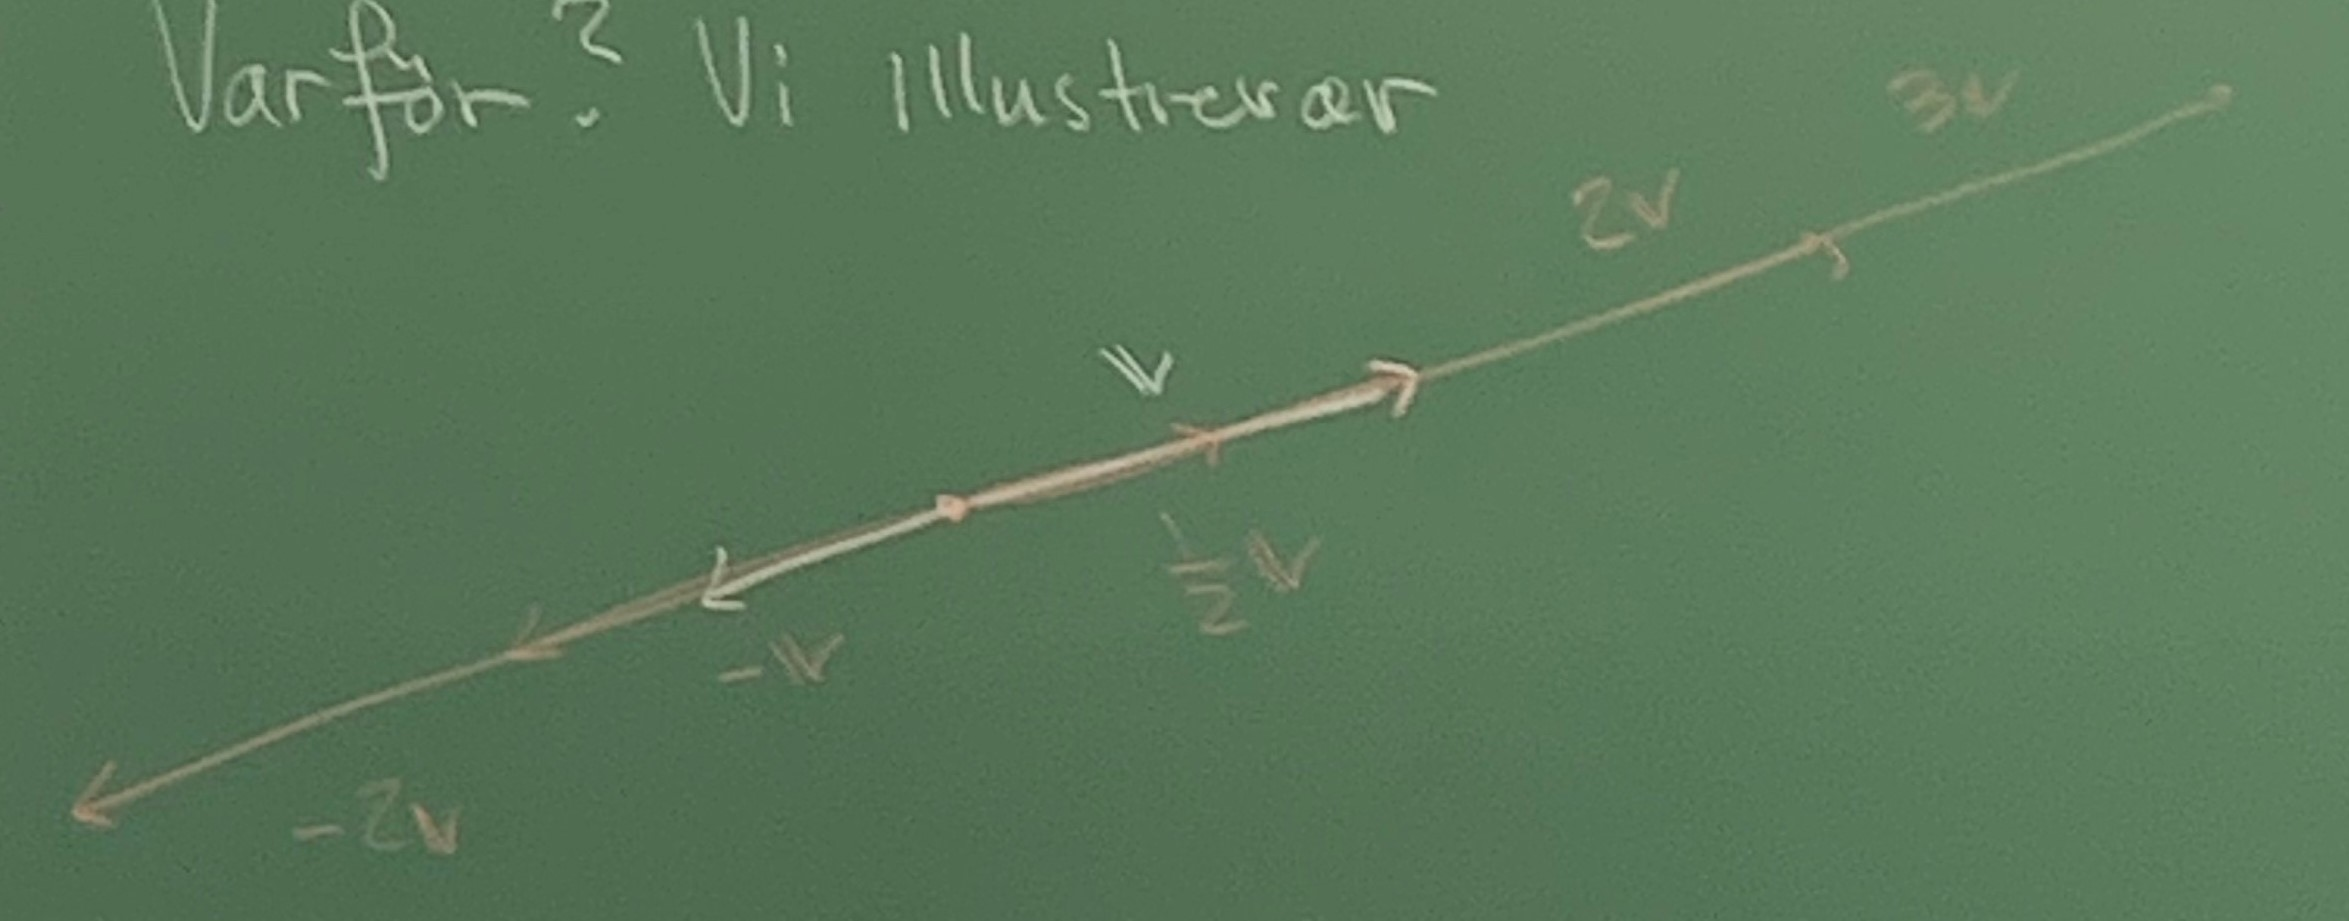
\includegraphics[scale=0.13]{imgs/22-01-20-img01.jpg}
    \\Varje sådan vektor $\bm{v}$ kallas för en \underline{riktningsvektor för linjen}.
    
    \paragraph{Ex} Vi säger att två vektorer $\bm{u}$ och $\bm{v}$ är \underline{parallella} om de har samma eller motsatt riktning. 
    Låt $\bm{u}$ och $\bm{v}$ vara två nollskilda och icke-parallella vektorer. Då är span(\{$\bm{u,v}$\})$=$span($\bm{u},\bm{v}$) ett plan. Varför?\\
    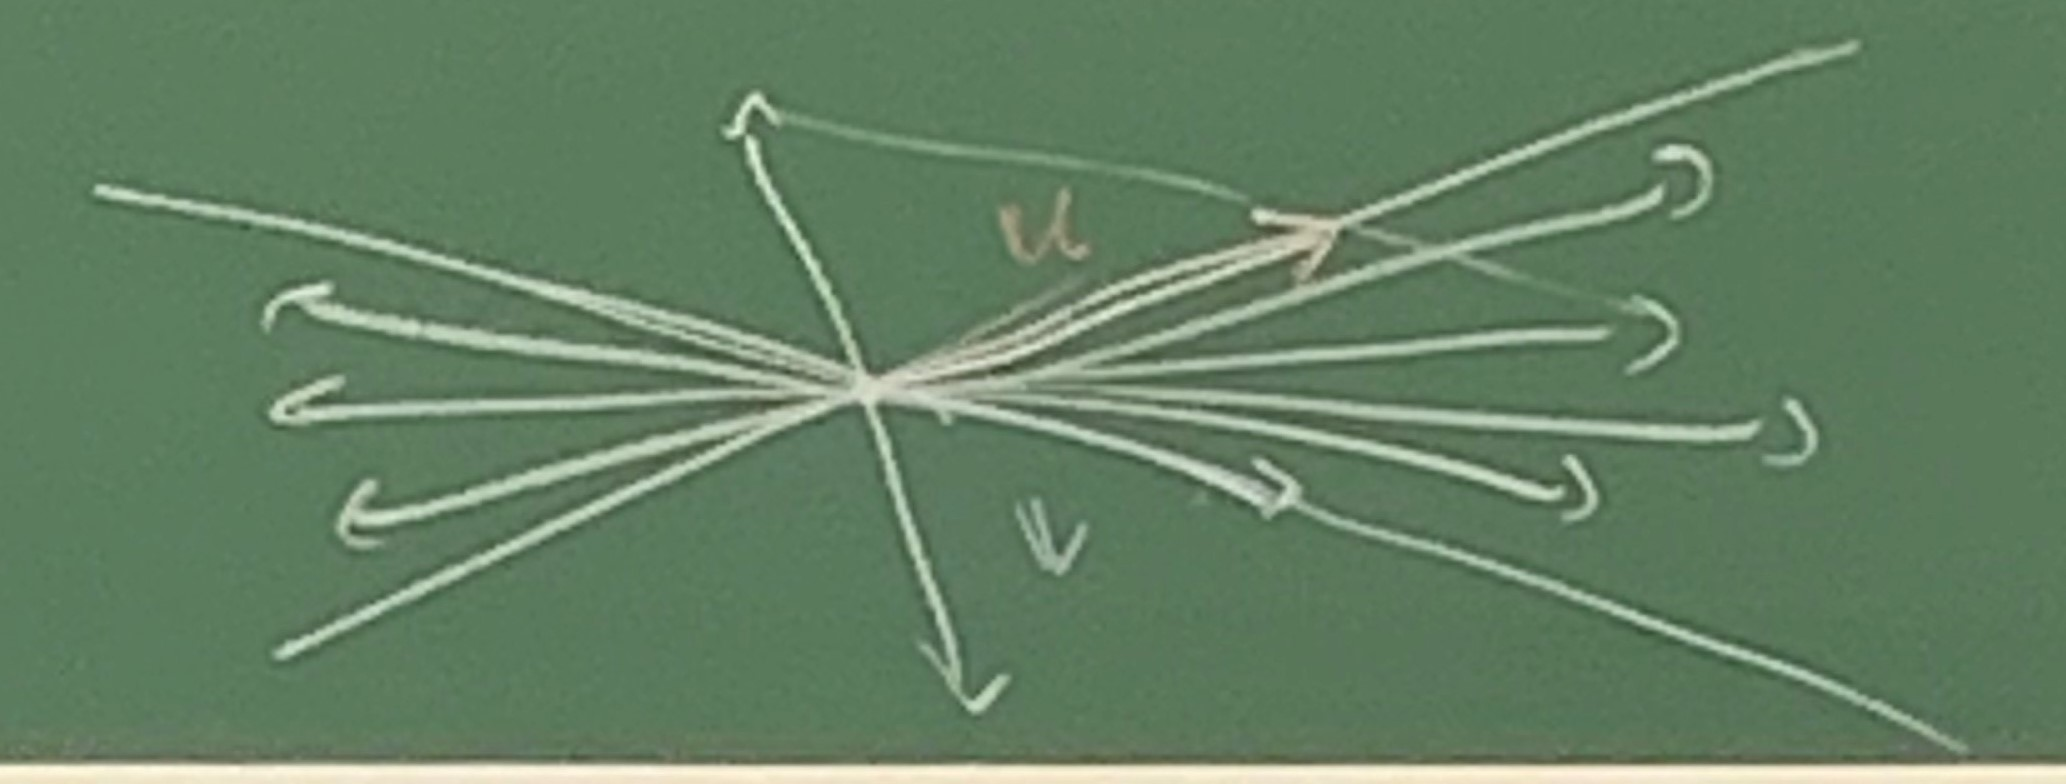
\includegraphics[scale=0.15]{imgs/22-01-20-img02.jpg}
    
\section{Skalärprodukten}
    \paragraph{Definition} Låt $\bm{u}$ och $\bm{v}$ vara två vektorer och låt $\alpha$ vara den minsta vinkeln mellan $\bm{u}$ och $\bm{v}$.
    Vi definierar skalärprodukten av $\bm{u}$ och $\bm{v}$ genom \\
    $\bm{u}\cdot \bm{v}=||\bm{u}||\cdot ||\bm{v}||cos(\alpha)$. 
    \\Observera att $\bm{u}\cdot \bm{v}$ är ett tal (en skalär).
    
    \paragraph{Ex} $\bm{u}\cdot \bm{u}=||\bm{u}||^{2}cos(0)=||\bm{u}||^{2}$
    
    \paragraph{Ex} Vi har att (antag att $\bm{u}$ och $\bm{v}$ är nollskilda)\\
    $\bm{u}\cdot \bm{v} = 0 \Leftrightarrow $ $\bm{u}$ och $\bm{v}$ är ortogonala (vinkelräta)
    
    \paragraph{Lösning} $\bm{u}\cdot \bm{v}=0 \Leftrightarrow ||\bm{u}||\cdot ||\bm{v}||cos(\alpha)=0 \Leftrightarrow cos(\alpha)=0 \Leftrightarrow $\\
    $\Leftrightarrow \alpha = \frac{\pi}{2} \Leftrightarrow bm{u}, \bm{u}$ ortogonala
    
    \paragraph{Proposition 1.16} Låt $\bm{u}$ och $\bm{v}$ vara nollskilda vektorer och låt $alpha$ vara vinkeln mellan dem.
    då gäller att 
    \begin{itemize}
        \item $\bm{u} \cdot \bm{v} > 0 \Leftrightarrow \alpha$ spetsig
        \item $\bm{u} \cdot \bm{v} = 0\Leftrightarrow \alpha$ rät
        \item $\bm{u} \cdot \bm{v} < 0\Leftrightarrow \alpha$ trubbig
    \end{itemize}
    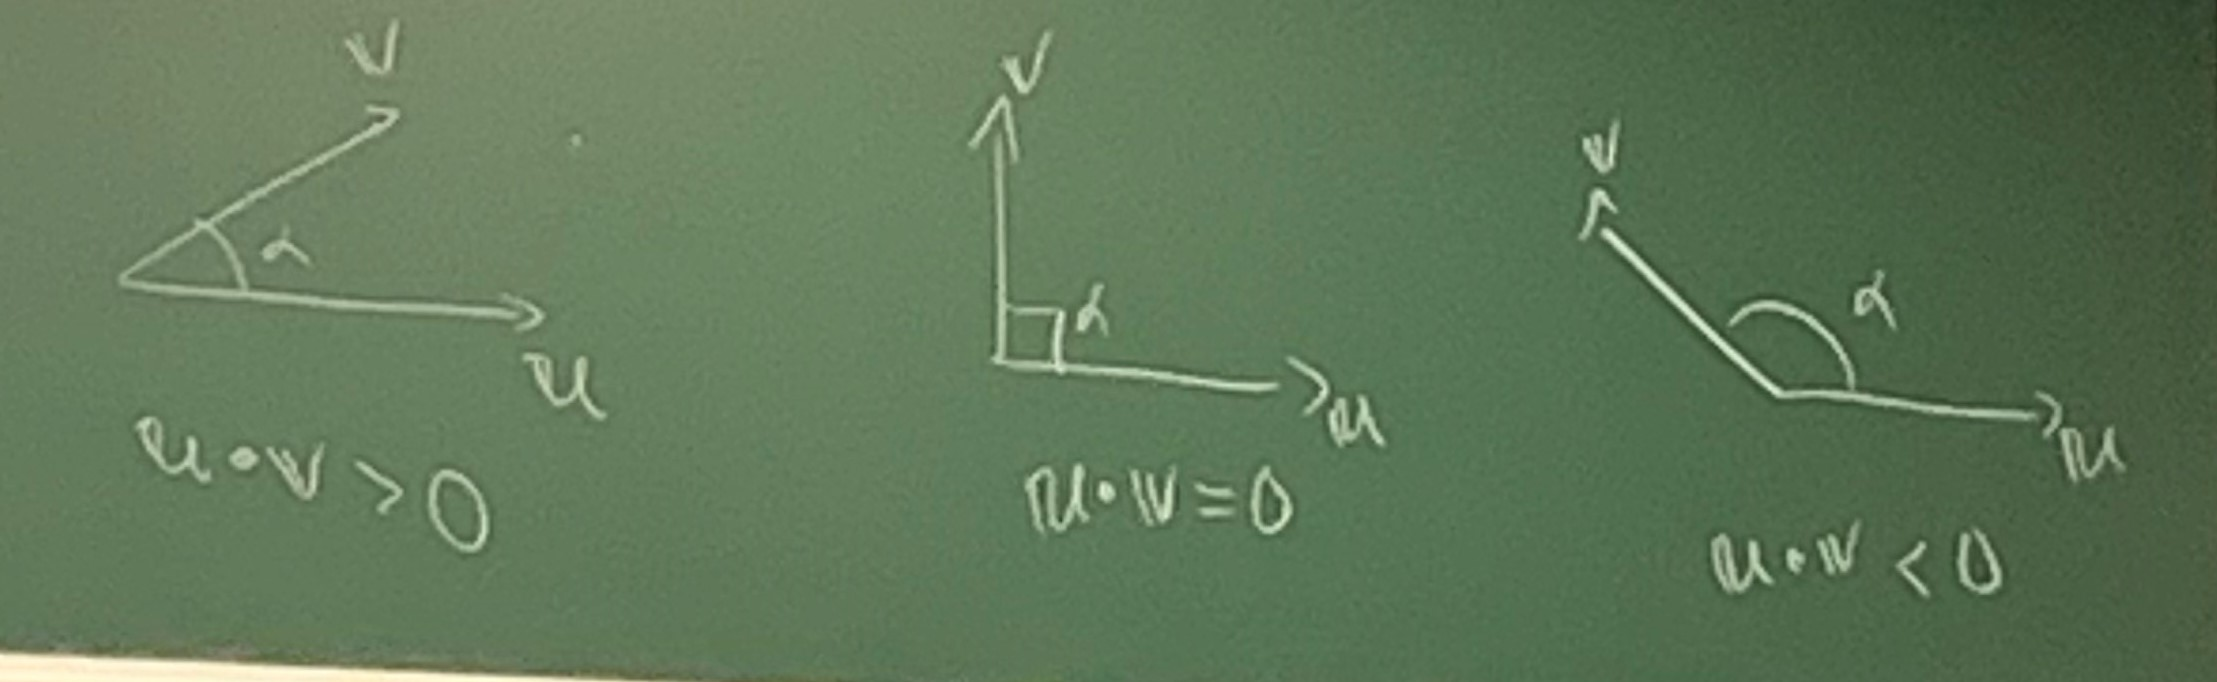
\includegraphics[scale=0.15]{imgs/22-01-20-img03.jpg}
    \subparagraph{Bevis} Eftersom $\bm{u} \cdot \bm{v} = ||\bm{u}|| \cdot ||\bm{v}||cos(\alpha)$ så har $\bm{u} \cdot \bm{v}$ samma tecken som $cos(\alpha)$.
    Så 
    \begin{itemize}
        \item $\bm{u} \cdot \bm{v} > 0 \Leftrightarrow cos(\alpha) > 0$
        \item $\bm{u} \cdot \bm{v} = 0 \Leftrightarrow cos(\alpha) = 0$
        \item $\bm{u} \cdot \bm{v} < 0 \Leftrightarrow cos(\alpha) < 0$
    \end{itemize}
    Påståendet följer av egenskaper för cosinus. $cos(\alpha) > 0 \Leftrightarrow 0 < \alpha < \frac{\pi}{2}$
    
    \paragraph{Definition} Låt $\bm{v}$ vara en vektor och L en linje. 
    \underline{Den ortogonala projektionen av $\bm{v}$ på L} är den vektor $\bm{v}_{L}$ som är parallell med L och så att $\bm{v}-\bm{v}_{L}$ är ortognal med L.\\
    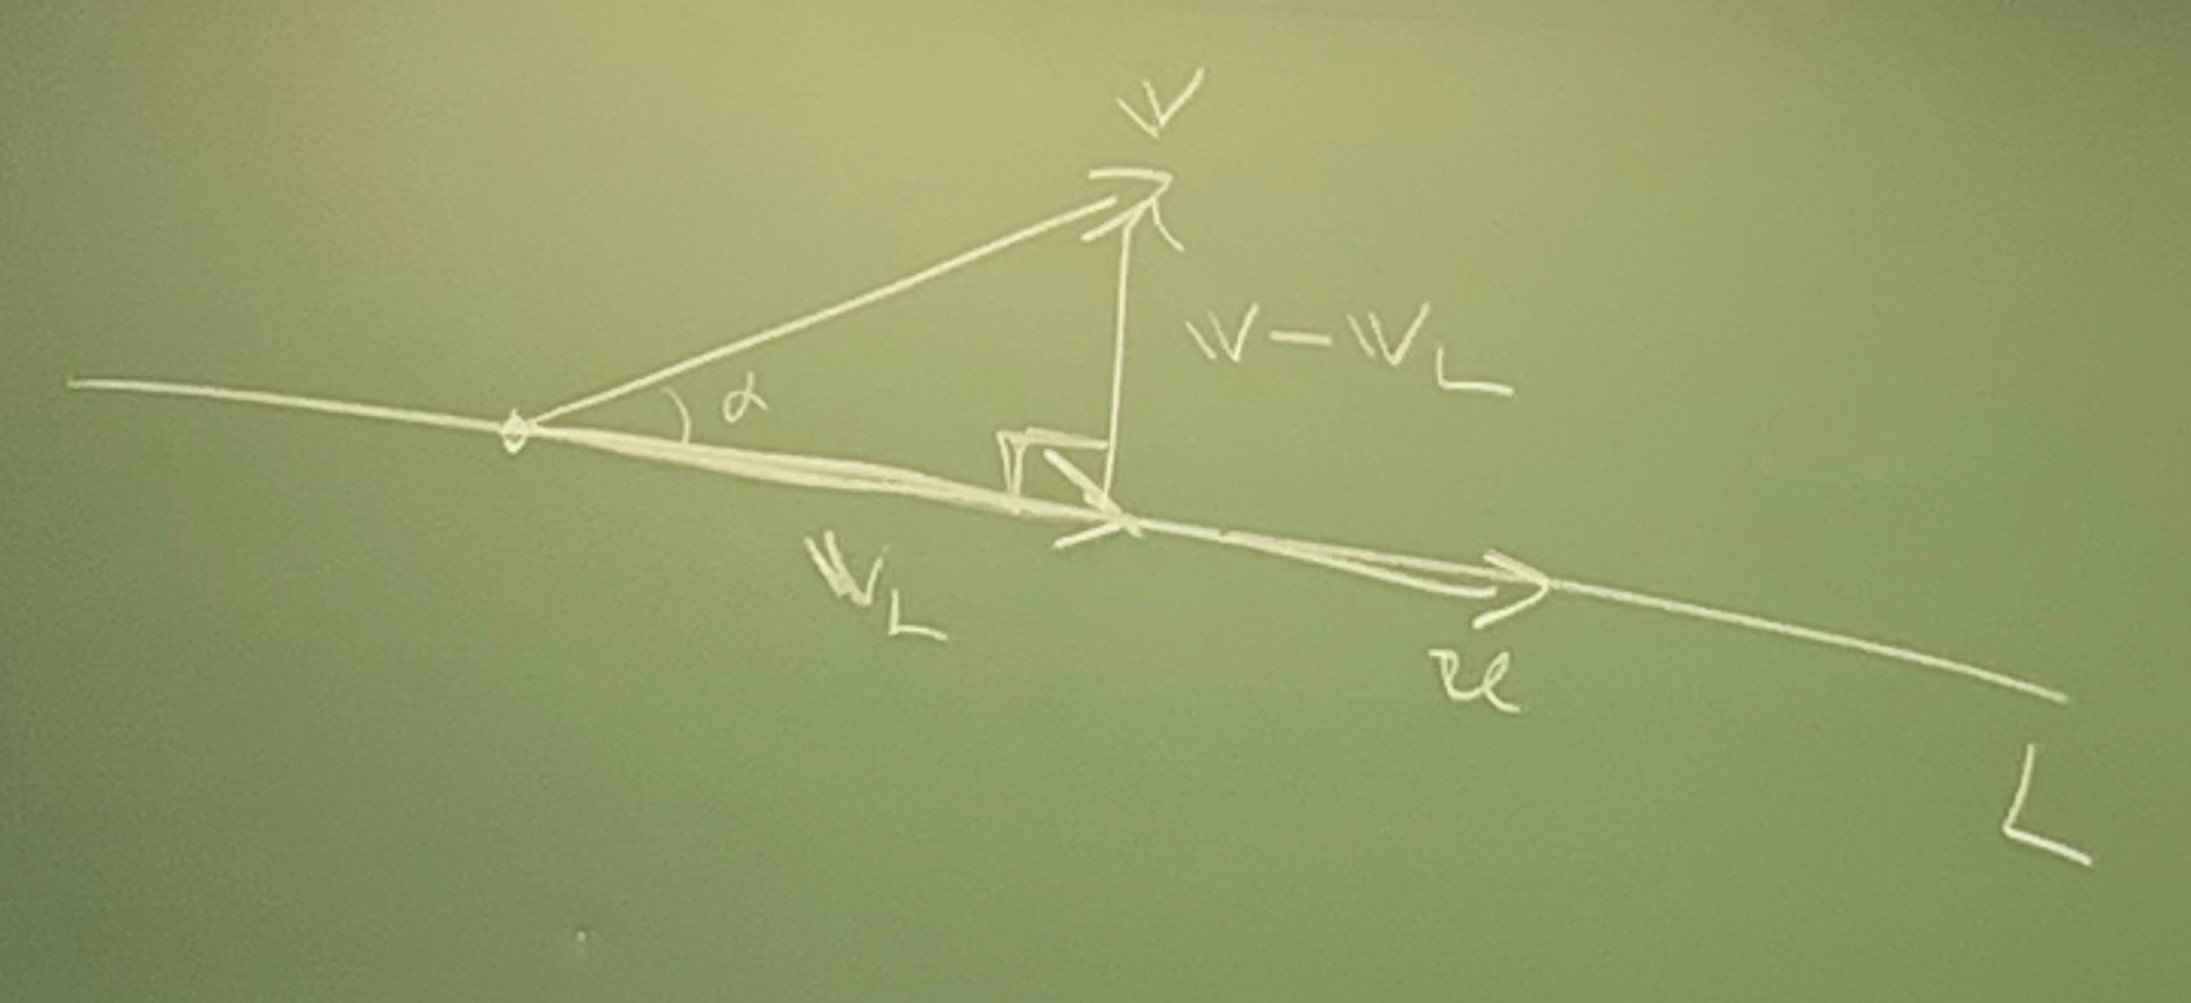
\includegraphics[scale=0.15]{imgs/22-01-20-img04.jpg}
    
    \paragraph{Proposition 1.18} Låt $\alpha$ och $\bm{v}$ vara vektorer och L en linje med riktningsvektor $\bm{u}$. 
    Då gäller att $\bm{u}\cdot \bm{v} = \bm{u} \cdot \bm{v}_{L}$
    \subparagraph{Bevis} Låt $\alpha$ vara vinkeln mellan $\bm{u}$ och $\bm{v}$.
    Antag att $\alpha$ är spetsig. Då $cos(\alpha)=\frac{||\bm{v}_{L}||}{||\bm{v}||}$.\\
    Vi får $\bm{u}\cdot \bm{v}=||\bm{u}||\cdot ||\bm{v}||cos(\alpha) = ||\bm{u}||\cdot ||\bm{v}||\cdot \frac{||\bm{v}_{L}||}{||\bm{v}||}=||\bm{u}||\cdot ||\bm{v}_{L}||cos(0)=\bm{u}\cdot\bm{v}_{L}$ v.s.b
    
    \paragraph{Proposition 1.19}
    \begin{enumerate}
        \item $\bm{u}\cdot \bm{v}=\bm{v}\cdot \bm{u}$
        \item $(c\bm{u})\cdot \bm{v} = c(\bm{u}\cdot \bm{v})$
        \item $\bm{u}\cdot (\bm{v} + \bm{w}) = \bm{u}\cdot \bm{v} + \bm{u} \cdot \bm{w}$
    \end{enumerate}
    
    \paragraph{Sats 1.20} Låt $\bm{u}$ vara en riktningsvektor för linjen L.
    Då gäller att $\bm{v}_{L} = \frac{\bm{u}\cdot \bm{v}}{\bm{u}\cdot \bm{u}}\bm{u}$ och $||\bm{v}_{L}||=\frac{|\bm{u}\cdot \bm{v}|}{||\bm{u}||}$.
    Illustration: \\
    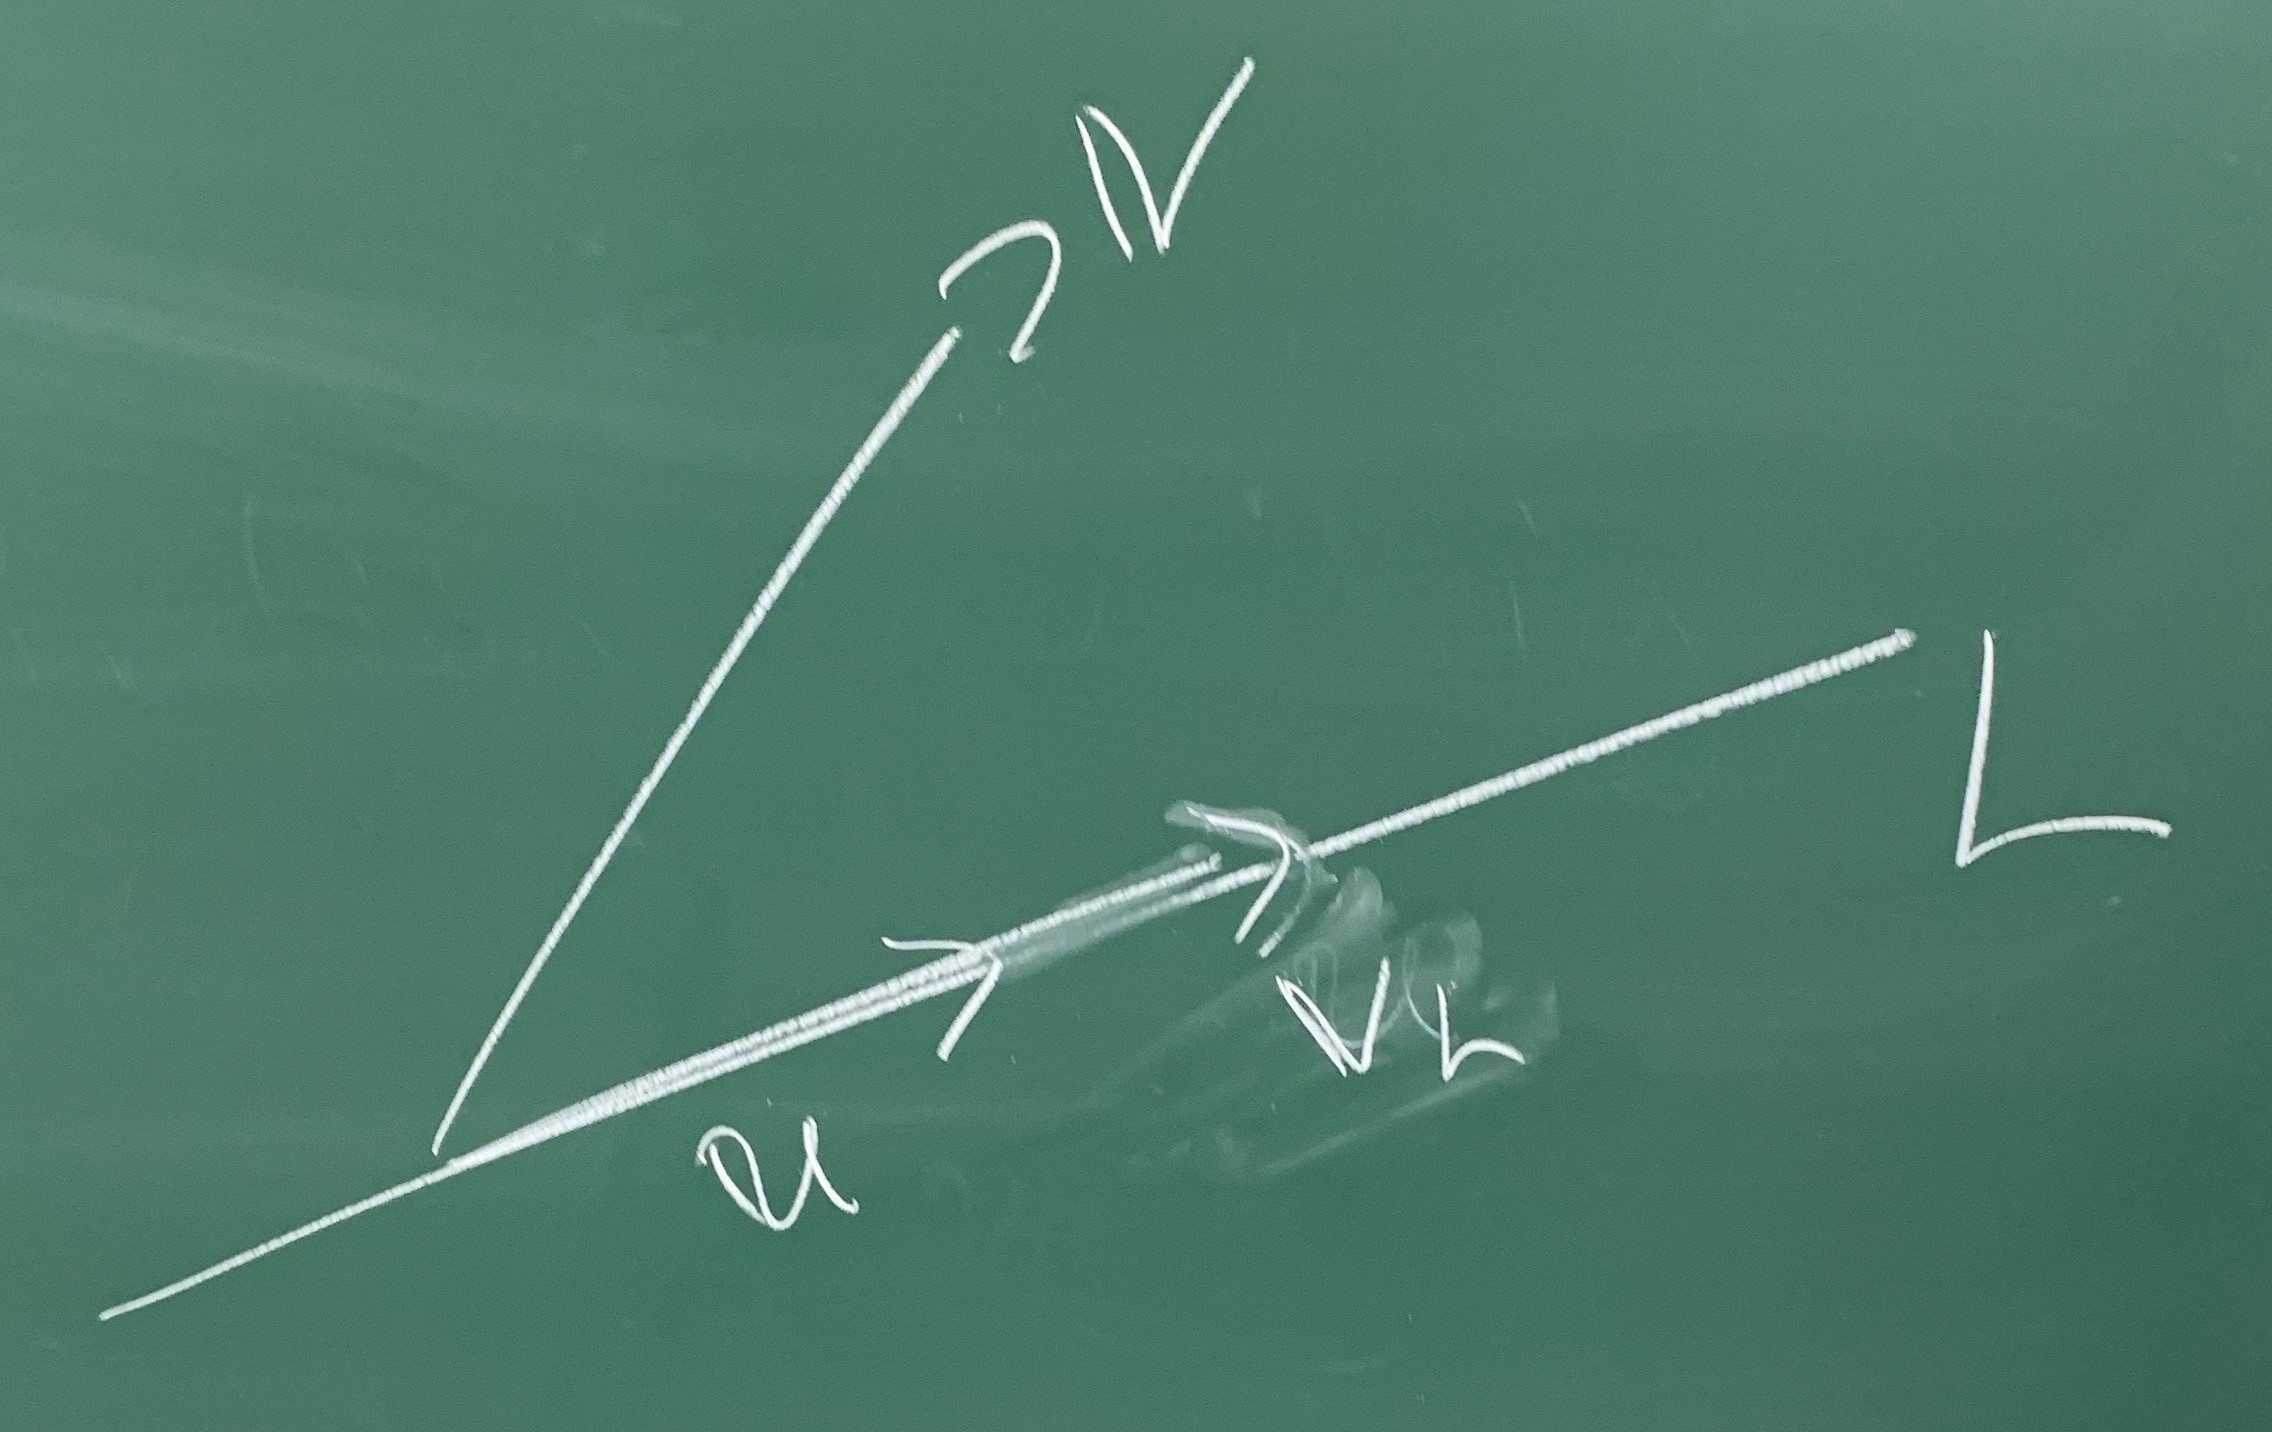
\includegraphics[scale=0.10]{imgs/22-01-20-img05.jpg}
    \subparagraph{Bevis} Vi vet att $\bm{v}_{L}$ och $\bm{u}$ är parallella och därför $\bm{v}_{L}=t\bm{u}$ för något $t\in \mathbb{R}$.
    $\bm{u}\cdot \bm{v}=\bm{u}\cdot \bm{v}_{L}=\bm{u}\cdot (t\bm{u}) \Rightarrow t=\frac{\bm{u}\cdot \bm{u}}{\bm{u}\cdot \bm{u}}$.
    \\Alltså
    $\bm{v}_{L}t\bm{u}=\frac{\bm{u}\cdot \bm{v}}{\bm{u}\cdot \bm{u}}\bm{u}$ och
    $||\bm{v}_{L}||=||\frac{\bm{u}\cdot \bm{v}}{\bm{u}\cdot \bm{u}}\bm{u}||=\frac{|\bm{u}\cdot v}{||\bm{u}||u^{2}}||\bm{u}||=\frac{|\bm{u}\cdot \bm{v}|}{||\bm{u}||}$
    
    \paragraph{Definition} \begin{itemize}
        \item En nollskild vektor $\bm{n}$ är en \underline{normal} till ett plan $\pi$ om $\bm{n}\cdot \bm{v} = 0$ för alla vektorer $\bm{v}$ som ör parallella med planet.\\
            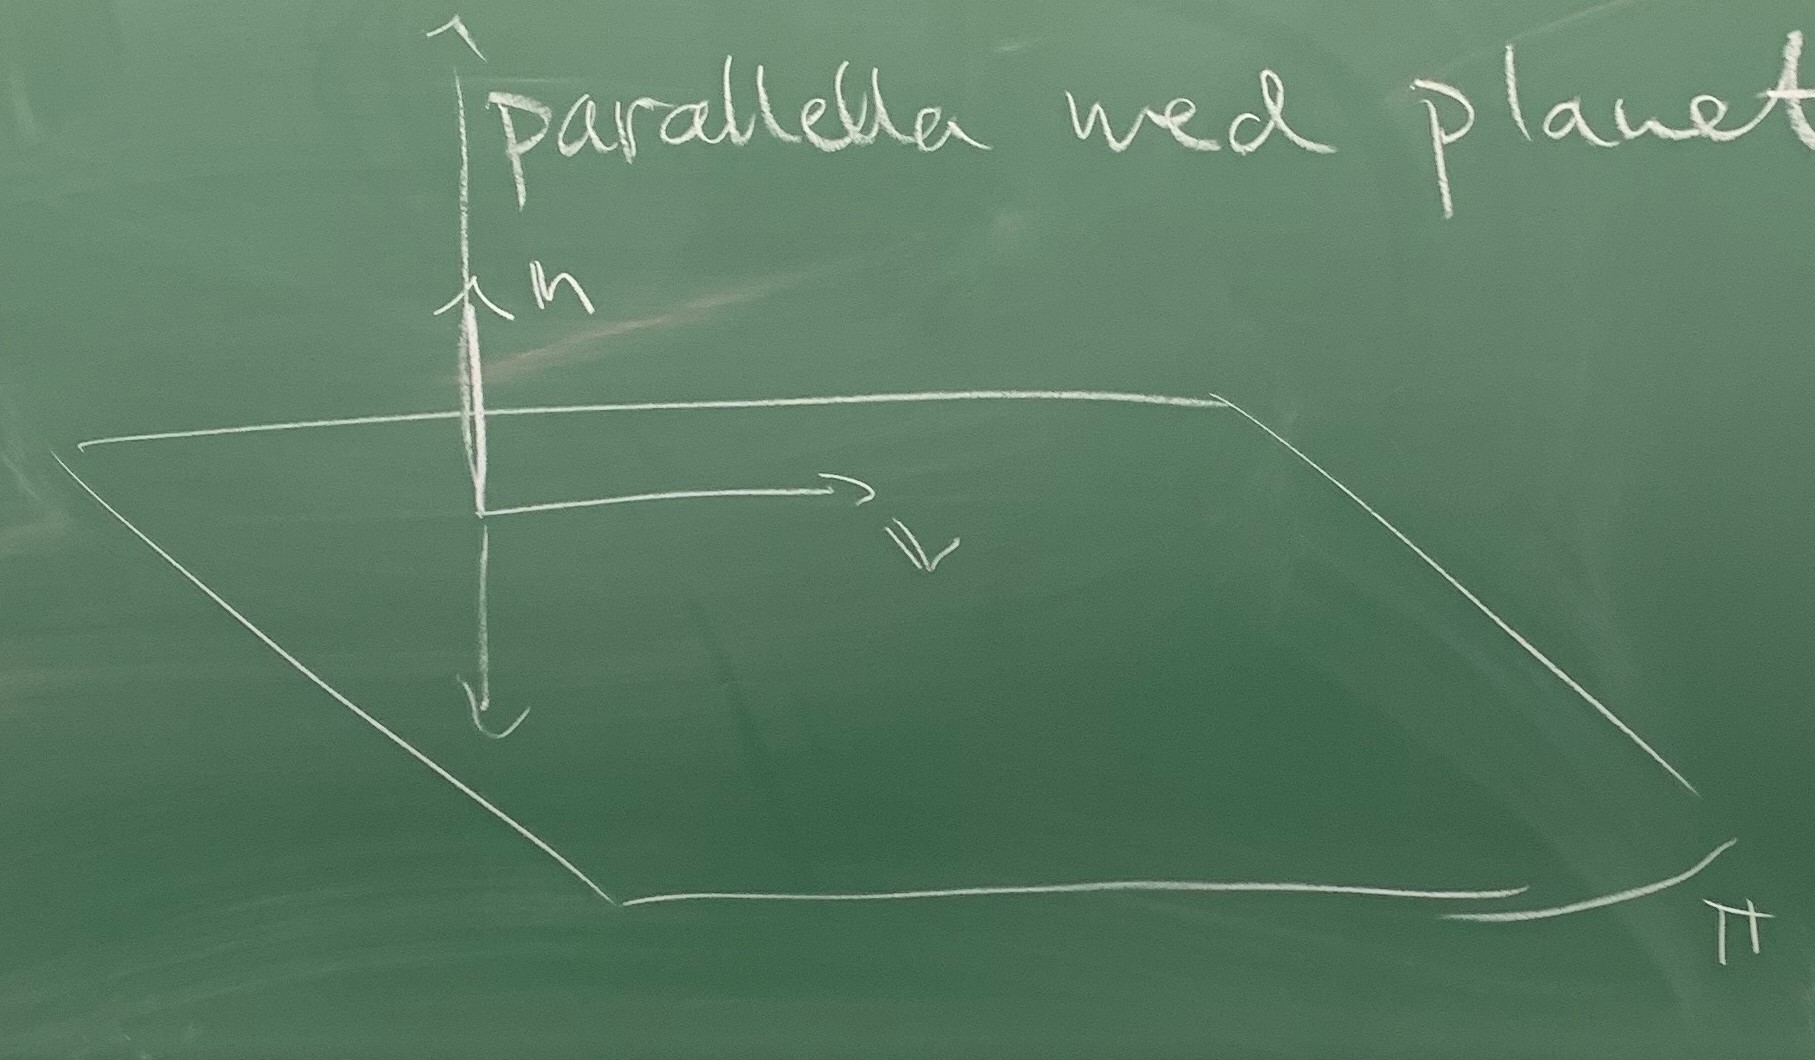
\includegraphics[scale=0.15]{imgs/22-01-20-img06.jpg}
        \item Givet en vektor $\bm{v}$ så är \underline{den ortogonala projektionen av $\bm{v}$ på $\pi$}, $\bm{v}_{\pi}$, den vektor i planet så att $\bm{v}-\bm{u}_{\pi}$ är en normal till $\pi$.\\
            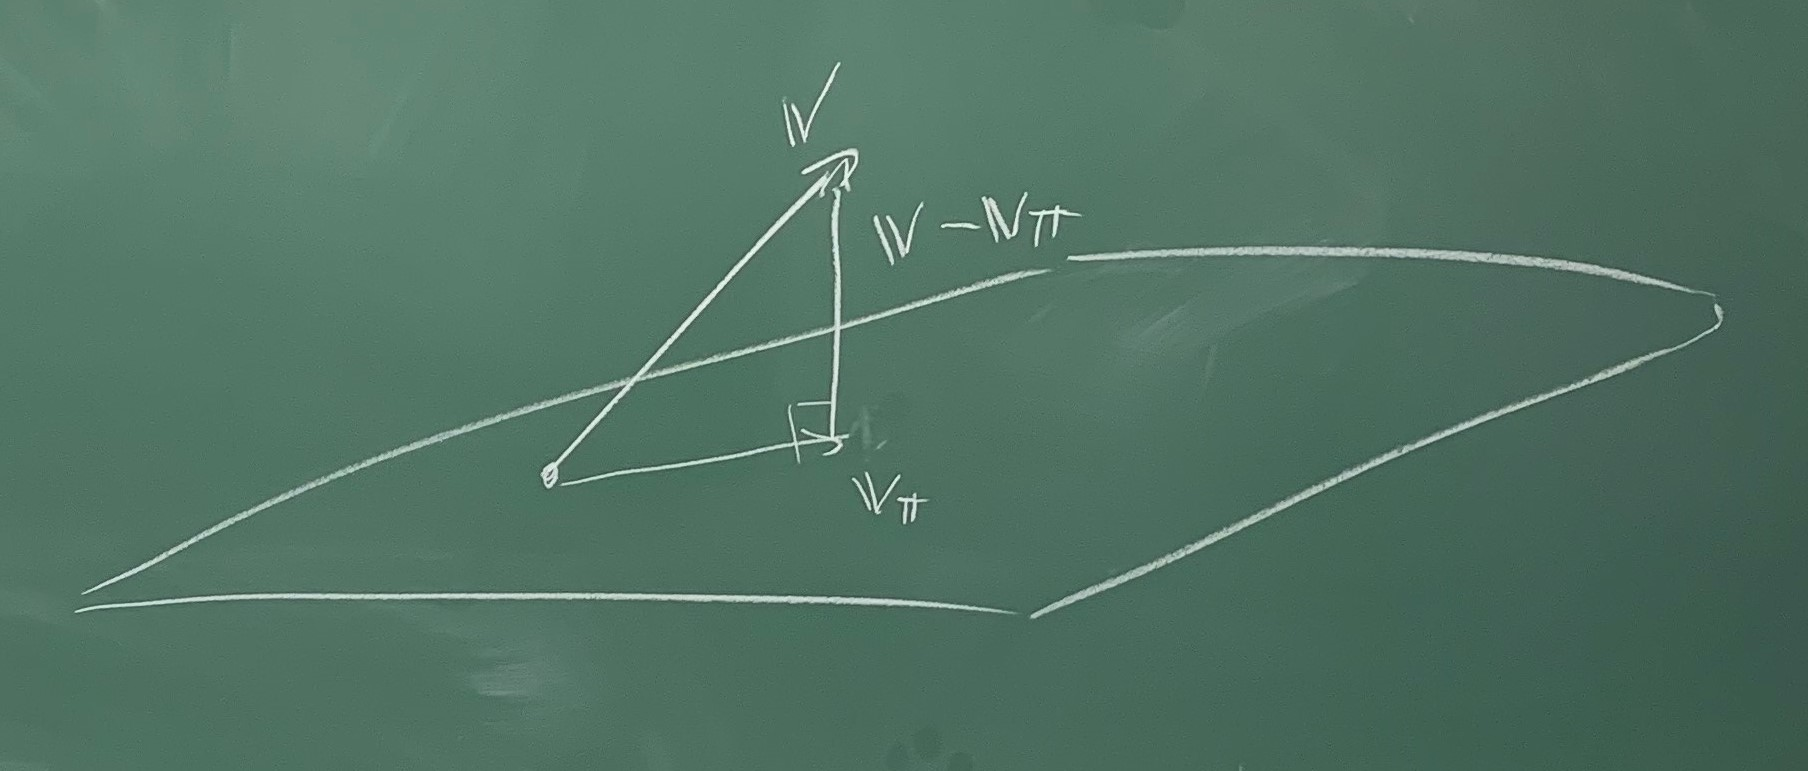
\includegraphics[scale=0.15]{imgs/22-01-20-img07.jpg}
    \end{itemize}
    
    \paragraph{Proposition 1.23} $(\bm{u} + \bm{u})_{\pi}=\bm{u}_{\pi} + \bm{v}_{\pi}$ (Inget bevis den här gången)

\section{Vektorprodukten}
    När vi studerar vektorprodukter är det viktigt att våra vektorer är i rummet.
    
    \paragraph{Definition} En vektortrippel $(\bm{u}, \bm{v}, \bm{w})$ sägs vara höger-orienterad om vyn från $\bm{w}$:s spets ger att den minsta vinkeln mellan $\bm{u}$ och $\bm{v}$ get att $\bm{u}$ vrids moturs mot $\bm{v}$.
    Annars sägs trippeln vara \underline{vänsterorienterad}.
    \\
    Givet två vektorer $\bm{u}$ och $\bm{v}$ så spänner de ett plan. Vi kan även se det som att de spänner ett parallellogram\\
    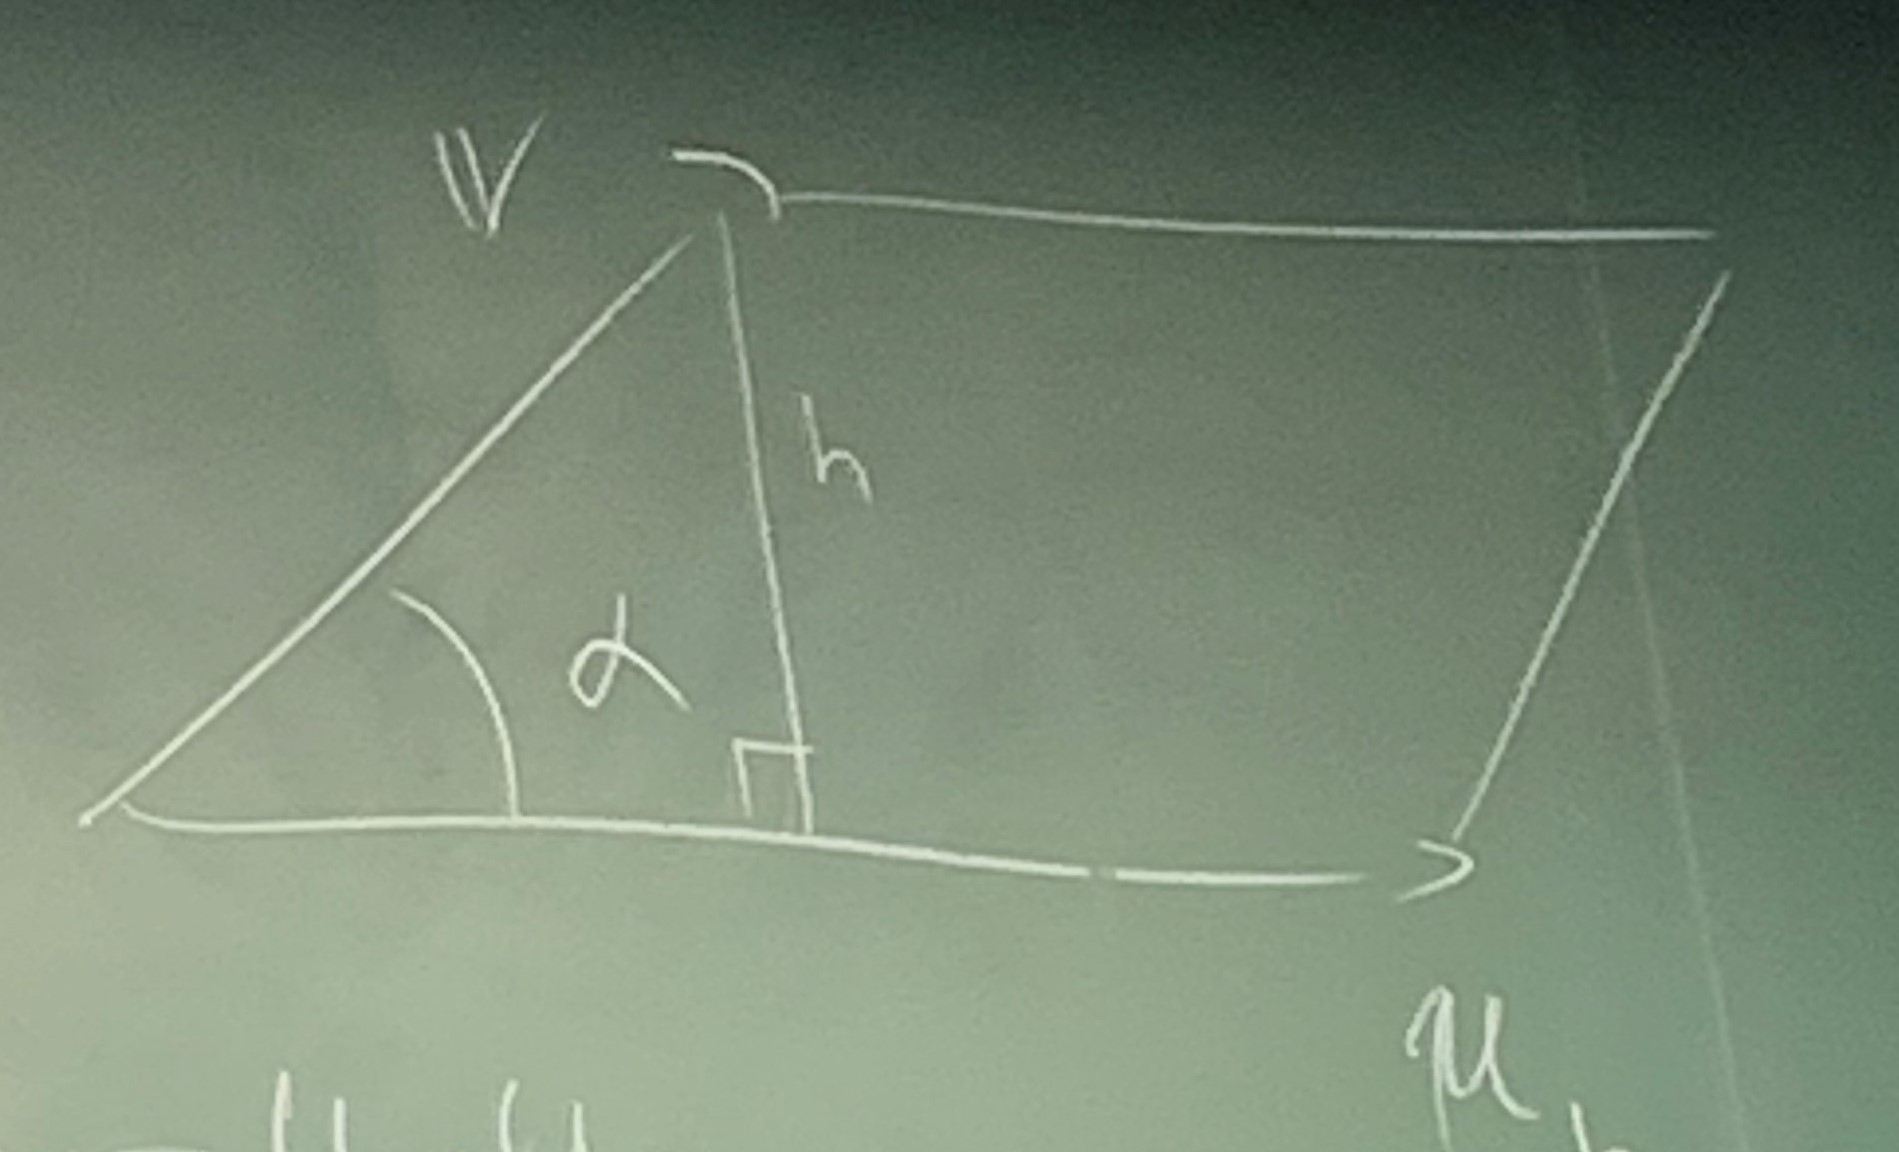
\includegraphics[scale=0.12]{imgs/22-01-20-img08.jpg}
    \\Arean av detta parallellogram är $||\bm{u}||\cdot||\bm{v}||sin(a)$.
    
    \paragraph{Definition} Låt $\bm{u}$ och $\bm{v}$ vara två vektorer. Vektorprodukten (kryssprodukten) av dem är vektorn $\bm{u}\times \bm{v}$ så att 
    \begin{enumerate}
        \item $\bm{u}\times \bm{v} = 0$ om $\bm{u}$,$\bm{v}$ är parallella
        \item $||\bm{u}\times \bm{v}||=||\bm{u}||\cdot ||\bm{v}||sin(a)$ 
        \item $\bm{u}\times \bm{v}$ är ortogonal mot $\bm{u}$ och $\bm{v}$
        \item $(\bm{u},\bm{v}, \bm{u}\times \bm{v})$ är högerorienterad.
    \end{enumerate}
    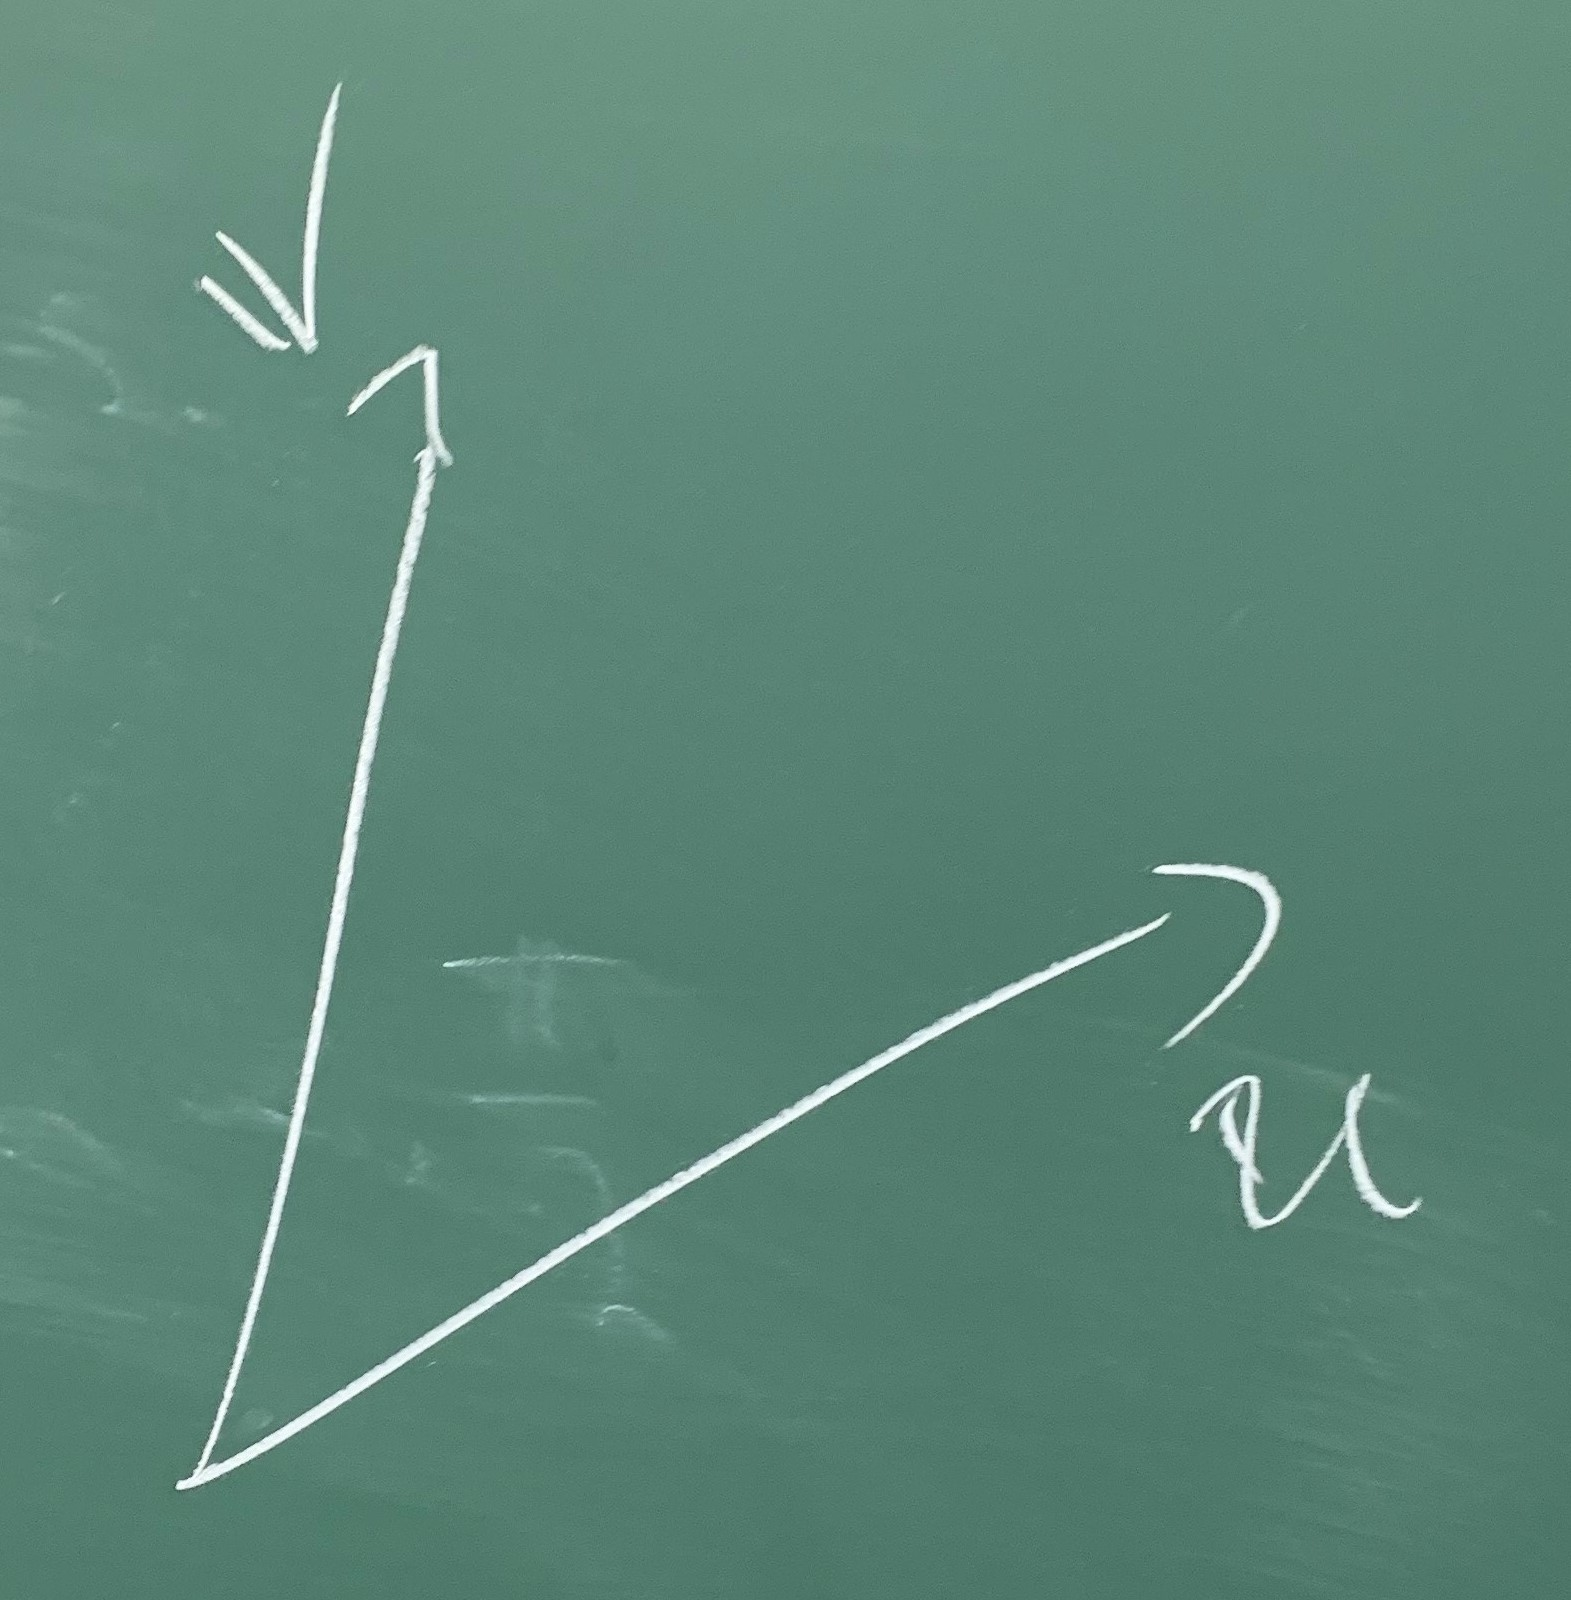
\includegraphics[scale=0.10]{imgs/22-01-20-img09.jpg}